\documentclass[twoside, 11pt, a4paper]{scrreprt}

\author{Lucas Hirschfeld}
\title{X-ray photoelectron spectroscopy (XPS) of Quinacridone (QA) on Ag(100)}
\date{\today}

\usepackage{fontspec}
\usepackage{polyglossia}
\setdefaultlanguage{english}

\usepackage[all]{nowidow}
\usepackage{amsmath,amsthm,amssymb,bm}
\usepackage{graphicx}
\usepackage{caption, booktabs, ltablex}
\usepackage{subcaption}
\usepackage{tabulary}
\usepackage{multirow}
\usepackage{chngcntr}
\usepackage{float}
\usepackage{microtype}
\usepackage{csquotes}
\usepackage[hidelinks, unicode]{hyperref}

% Bibliographie-Einstellungen
\usepackage[backend=biber,
    citestyle=numeric-comp,
    bibstyle=numeric,
    bibwarn=true,
    autocite=superscript,
    abbreviate=true, 
    sorting=none, 
    url=false, 
    doi=false,
    eprint=false,
    isbn=false]{biblatex}
\addbibresource{literature.bib}

% Custom cite command
\DeclareCiteCommand{\supercite}[\mkbibsuperscript]%
{\usebibmacro{cite:init}%
    \let\multicitedelim\supercitedelim%
    \iffieldundef{prenote}%
    {}%
    {\BibliographyWarning{Ignoring prenote argument}}%
    \iffieldundef{postnote}%
    {}%
    {\BibliographyWarning{Ignoring postnote argument}}%
    \bibleftbracket%
}%
{\usebibmacro{citeindex}%
    \usebibmacro{cite:comp}}
{}%
{\usebibmacro{cite:dump}%
    \bibrightbracket%
}

\usepackage{acronym}
\usepackage{scrhack}
\usepackage[version=4]{mhchem}

% Tabellen-Einstellungen
\usepackage{booktabs}
\belowrulesep=0em
\aboverulesep=0em
\usepackage{hhline}

% SI-Einheiten
\usepackage{siunitx}
\DeclareSIUnit\angstrom{\text{Å}}
\DeclareSIUnit\atomicmassunit{u}

% Seitenstil
\usepackage{scrlayer-scrpage}
\clearpairofpagestyles
\ihead{\leftmark}
\ohead{\rightmark}
\ofoot*{\pagemark}
\cfoot*{}
\pagestyle{scrheadings}
\addtokomafont{pageheadfoot}{\normalfont}

\renewcommand*{\chaptermarkformat}{\thechapter.\ }
\renewcommand*{\sectionmarkformat}{\thesection.\ }

% Layout-Einstellungen
\newcommand{\mylinespread}{1.5}
\setlength{\parindent}{0em}

\begin{document}
\KOMAoptions{twoside=false}
\begin{titlepage}
	\centering
	{\scshape\LARGE \par}
	\vspace{1cm}
	{\huge\bfseries \textsf{\Acf{XPS} of \Acf{QA} on the Ag(100) surface}\par}
	\vspace{3 cm}
	{\Large\bfseries Focusing Laboratory Course \par}
	\vspace{3cm}
    {\large Lucas Hirschfeld\par}
	\vspace{3cm}
    {\large Clausius Institute for Physical and Theoretical Chemistry
	University of Bonn\par}
	\vspace{2.5cm}
    {\large Research group of Prof. Dr. Moritz Sokolowski\par}
	\Acf{XPS} of \Acf{QA} on the Ag(100) surface
	\vfill
	{\large Bonn
	\the\year{}}
\end{titlepage}

\KOMAoptions{twoside=true, DIV=last, BCOR=8.25mm}

\cleardoublepage

\thispagestyle{empty}
\pagenumbering{gobble}
\tableofcontents
\cleardoublepage
\pagenumbering{arabic}
\chapter{Introduction}

The interface of organic semiconductors with metal surfaces is of particular importance within the domain of organic electronic devices. The aforementioned electronic devices include, for example, \acp{OLED},\autocite{Wang2012, Facchetti2007} \acp{OFET}\autocite{Kulkarni2004, Shahnawaz2019} and \acp{OPV}.\autocite{Hains2010} A significant number of investigations into these interfaces have focused on the structural characteristics of the organic semiconductors, which are imperative for the functionality of the devices. Consequently, organic molecules with a large $\pi$-conjugtated system are frequently utilized, as they demonstrate high electron and hole mobilities.

Moreover, the property of 1D molecular chain formation is of significance for atomic and molecular wires. These wires are important components for modern devices, including those employed in computing, energy storage, photonics, photovoltaics and other applications.\autocite{Goktas2018, Zhou2019, Jia2019, Daniels2023, Gu2023, Patzsch2017, Imran2018} In addition, 1D structures are of considerable interest for the investigation of the physical properties of organic adsorbates. A comparison between 1D structures and structures with higher dimensionality can provide insights into the relation between individual atoms or molecules and the corresponding properties of the system.

One molecule that has been extensively studied in the context of electronic devices is \ac{QA}. \Ac{QA} is an organic, prochiral molecule with a large $\pi$-conjugated system, which has been shown to form well-defined structures on metal surfaces. In previous studies, the potential of \ac{QA} for application in electronic devices has been demonstrated.\autocite{Glowacki2013,DanielGlowacki2012, Wang2016} Its potential extends beyond the domain of printer toners, where it is generally employed, offering significant promise for applications in diverse fields. Examples of applications for \ac{QA} are \acp{OFET}\autocite{Jeon2018, Jeong2017, Kanbur2019, Berg2009}, \acp{OLED}\autocite{Wang2016a, Min2021, Cunha2018} and \acp{OPV}\autocite{Dunst2017, Sung2017}.

The well-defined structures of \ac{QA} consist of 1D molecular chains. These structures have been identified in the bulk crystal structure\autocite{Paulus2007} and on surfaces.\autocite{Humberg2024, Wagner2014, Trixler2007, Eberle2019} The formation of the 1D molecular chains is driven by intermolecular hydrogen bonds and the interaction with the adsorbate.\autocite{Humberg2024, Humberg2020}

For \ac{QA}, two distinct phases on Ag(100) have been identified. The initial phase is predominantly attributable to intermolecular hydrogen bonds, resulting in a 1D molecular chain structure that is not commensurate. The second phase is characterized by a decreased number of hydrogen bonds and is commensurate. The phase transition between these two phases is driven by the interaction with the substrate and the temperature.\autocite{Humberg2024, Humberg2020} The structure formation of \ac{QA} on Ag(100) in the distinct phases show the competition between the intermolecular hydrogen bonds and the interaction with the substrate.

As a result of the aforementioned phase behaviour of \ac{QA} on Ag(100), the molecule is of particular interest for the investigation of the structural characteristics. The formation of 1D molecular chains with intermolecular hydrogen bonds and the phase transition between two distinct phases provide a unique opportunity to study the interplay between intermolecular interactions and substrate interactions.

The objective of this research is to ascertain how the structure of \ac{QA} on Ag(100) is impacted by the interplay between intermolecular interactions via hydrogen bonds and substrate interactions of the molecule across the two distinct phases. Therefore, \ac{XPS} is employed as the primary technique, which provides insights into the electronic structure and chemical environment of the adsorbate. The investigation is conducted for both phases which allows the observation of the differences in these phases.

The measured \ac{XPS} spectra provide insight into the number of hydrogen bonds and the interaction with the substrate. The ratio of hydrogen bonds per molecule between the two phases has been determined as 2:1, contradicting the earlier report by N. Humberg, who stated a ratio of 2:1.5.\autocite{Humberg2024, Humberg2020} This prompts the necessity for a novel structure model, a subject that will be examined in the subsequent chapters.

\cleardoublepage
\chapter{Literature}
\section{Quinachridone (QA)}

The examined adsorbate \acf{QA} is a high symmetric, prochiral organic molecule with the full IUPAC name 5,12-dihydro-quino[2,3-\textit{b}]acridine-7,14-dione and the sum formula \ce{C20H12N2O2}. Organic crystals exhibit a color which can range from red to violet.\autocite{ChemicalBook2025,ChemSpider2025}

\ac{QA} is most prominently recognized as the parent structure of a group of pigments, most notably Pigment Violet 19 (C.I. 73900). This particular pigment is extensively utilized in industrial applications due to its remarkable color properties and stability.\autocite{ChemicalBook2025,ChemSpider2025} The molecular structure of \ac{QA} is shown in \autoref{fig:QA}.

\begin{figure}[H]
	\centering
	\begin{subfigure}[b]{0.48\linewidth}
		\centering
		\includegraphics[width=\linewidth]{images/QA.pdf}
		\caption{Skeletal structure}
	\end{subfigure}
	\hfill
	\begin{subfigure}[b]{0.48\linewidth}
		\centering
		\includegraphics[width=\linewidth]{images/QA_molecule.png}
		\caption{Ball-and-stick model}
	\end{subfigure}
	\caption{Molecular structure of \acf{QA}.}
	\label{fig:QA}
\end{figure}


The molecule is classified as a heterocyclic compound. Its structure is characterized by a conjugated ring system that imparts significant rigidity and planarity to the molecule.\autocite{forBiotechnologyInformation2025}. \ac{QA} is of the symmetry group $\mathrm{C_{2h}}$ and has a molar mass of 312.32~\si{g/mol}. The molecule is a crystalline solid with four known different crystal structures under standard conditions.\autocite{Paulus2007,Mizuguchi}


\section{Structures of Quinachridone (QA) on the Ag(100) surface}

For \ac{QA} deposited onto the Ag(100) surface, two structural phases were observed to form: the $\alpha$- and $\beta$-phase. A thorough examination of these two phases has been conducted by N. Humberg.\autocite{Humberg2024, Humberg2020}

The formation of the $\alpha$-phase occurs subsequent to the deposition of the \ac{QA} molecules onto the Ag(100) surface at a sample temperature of 300~\si{K}. This phase is composed of parallel molecular chains that are flat-lying with the $\pi$-system being oriented parallel to the Ag(100) surface. The \ac{QA} molecules are connected via intermolecular hydrogen bonds between the keto groups of one molecular chain and the amine groups of another, resulting in 2 hydrogen bonds per molecule. It was also determined that the domains under consideration are homochiral, a finding that suggests a high degree of mobility for the \ac{QA} molecules on Ag(100) surface at 300~\si{K}.

In addition, the superstructure matrix of the $\alpha$-phase for a complete \ac{ML} was determined using a \ac{SPA-LEED} image and \ac{STM} results. The following superstructure matrix was found
\begin{equation*}
\mathbf{M_\alpha} =\begin{pmatrix}
2 & 1.25 \\
-3 & 4.80 
\end{pmatrix},
\end{equation*}
which shows that the structure is of the \ac{POL} type. This means that every lattice point of the superstructure falls on a substrate lattice line of the [10] direction of the Ag(100) surface. It should be noted that the intermolecular distance $b_1$ between the molecules of a chain are determined by the intermolecular hydrogen bonds and does not change with the coverage. The distance between two molecular chains $b_2$ increases with decreasing coverage.

The \ac{STM} images, the \ac{SPA-LEED} image and the structure model of \ac{QA} on Ag(100) in the $\alpha$-phase is illustrated in \autoref{fig:literature_alpha}.
\begin{figure}[htb]
	\centering
	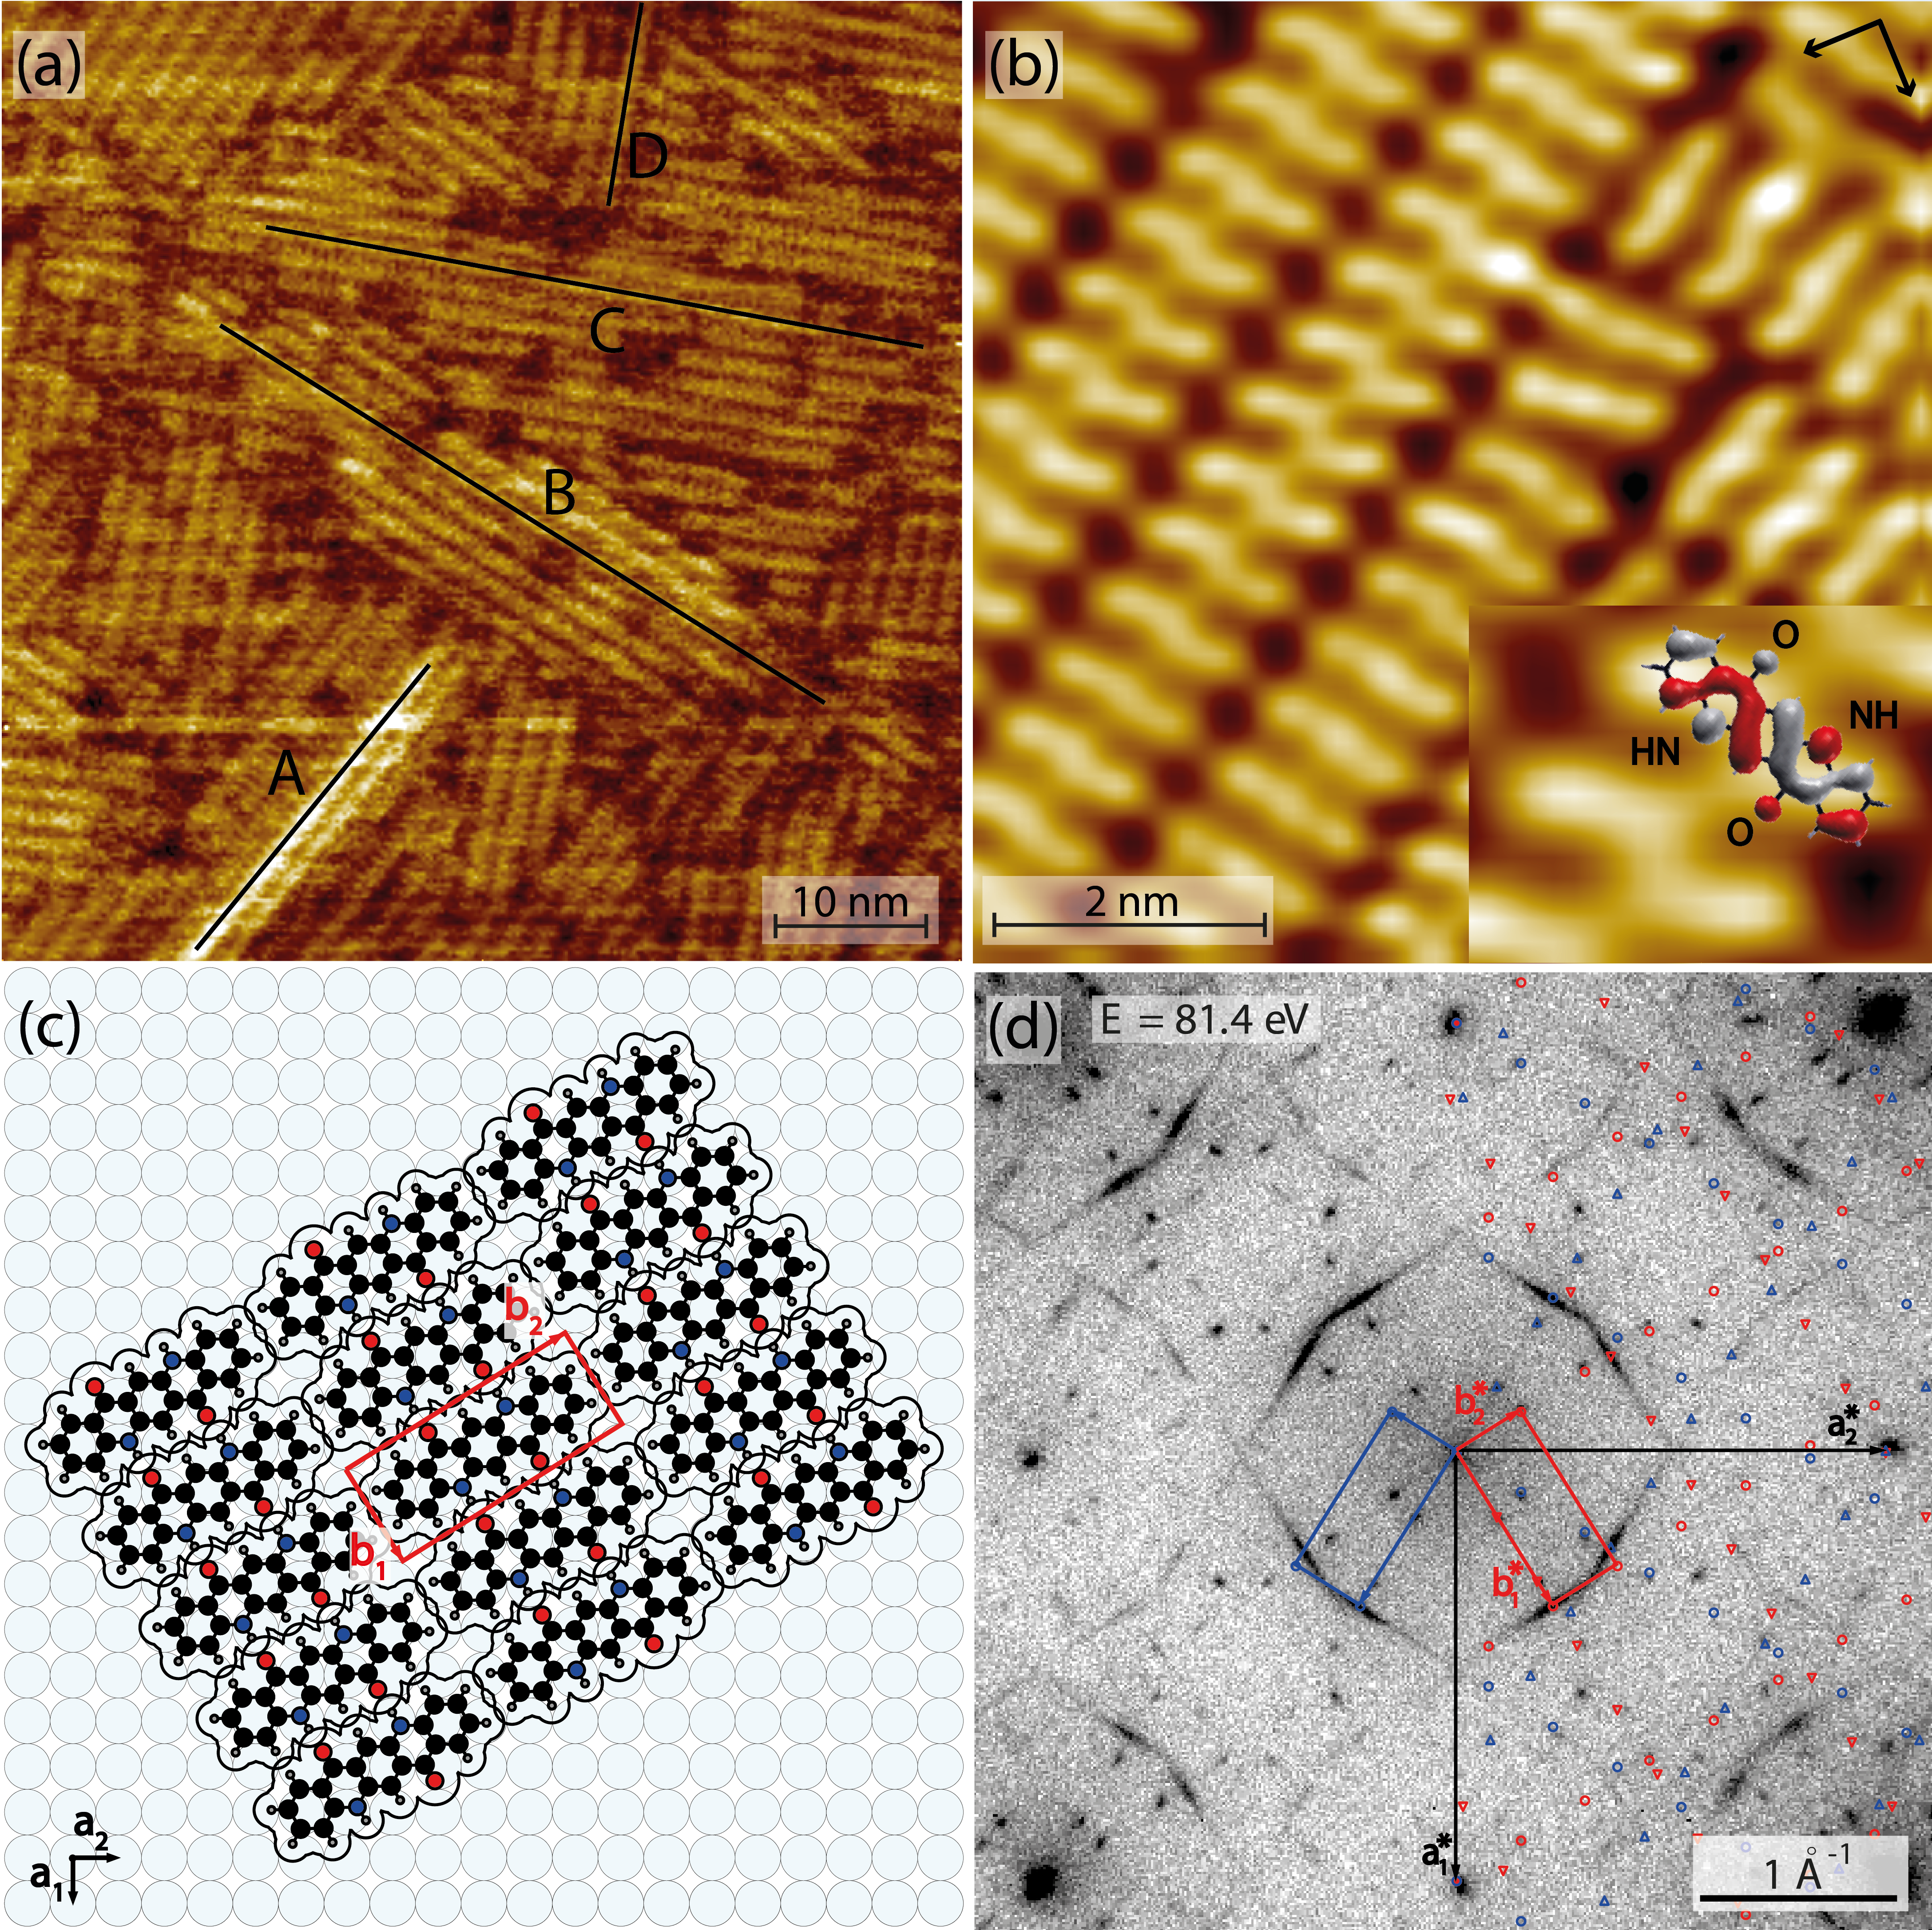
\includegraphics[width=0.7\textwidth]{images/literature_alpha.png}
	\caption{Structure of complete \ac{ML} of \ac{QA} on Ag(100) in the $\alpha$-phase. The image shows an overview \ac{STM} image (a), a close-up \ac{STM} image of the molecular arrangement (b), the \ac{SPA-LEED} image (c) and the structure model (d). The image is taken from reference \cite{Humberg2024}.}
	\label{fig:literature_alpha}
\end{figure}
The phase transition from the $\alpha$-phase to the $\beta$-phase occurs when the sample is heated up to 500~\si{K} for 15 minutes. The phase transition is irreversible. This means that the $\alpha$-phase is metastable and is stabilized by a kinetic barrier. This kinetic barrier corresponds to the energy required to break the hydrogen bonds between the \ac{QA} molecules in the $\alpha$-phase.

For the $\beta$-phase, the investigation revealed a 2D network of molecular chains, which are comprised of dimers and manifest periodic indents. The existing structure model proposes a single hydrogen bond between the dimers instead of theoretical two possible hydrogen bonds. The two molecules of the dimer form two hydrogen bonds with each other, resulting in 1.5 hydrogen bonds per molecule.

Once more, employing a \ac{SPA-LEED} image and \ac{STM} results, the superstructure matrix of the $\beta$-phase for a complete \ac{ML} was determined as
\begin{equation*}
\mathbf{M_\beta} =\begin{pmatrix}
4 & 3 \\
-5 & 3 
\end{pmatrix},
\end{equation*}
which means that the structure is commensurate. In comparison to the \ac{POL} type of the $\alpha$-phase, the commensurate structure of the $\beta$-phase indicates that the superstructure for the $\beta$-phase is aligned with the substrate in a way that the periodicity of the superstructure is a multiple of the substrate lattice constant. In general, the commensurate structure of the $\beta$-phase indicates a stronger interaction with the substrate and relates to energy gain compared to the $\alpha$-phase.\autocite{Hooks2001}

The \ac{STM} images, the \ac{SPA-LEED} image and the structure model of \ac{QA} on Ag(100) in the $\beta$-phase is illustrated in \autoref{fig:literature_beta}.
\begin{figure}[htb]
	\centering
	\includegraphics[width=0.7\textwidth]{images/literature_beta.png}
	\caption{Structure of complete \ac{ML} of \ac{QA} on Ag(100) in the $\beta$-phase. The image shows an overview \ac{STM} image (a), a close-up \ac{STM} image of the molecular arrangement (b), the \ac{SPA-LEED} image (c) and the structure model (d). The image is taken from reference \cite{Humberg2024}.}
	\label{fig:literature_beta}
\end{figure}
\cleardoublepage
\chapter{Theory}
\section{X-ray photoelectron spectroscopy (XPS)}

\Acf{XPS} is one of the different types of electron spectroscopy where an excitation leads to the ejection of an electron from a bound state to the continuum, called the photoelectric effect.\autocite{Hertz1887, Einstein1905} The photons of x-rays have similar energy as the \acfp{BE} of deep core electrons and are therefore used for the excitation. One can divide x-rays for surface science into two different categories: soft (100 - 2100~\si{\eV}) and hard x-rays (> 2100~\si{\eV}).

When an atom absorbs one of these photons, a photoelectron, which has a characteristic energy corresponding to the atom and its bonding environment, is emitted. The change of energy due to the bonding environment and its oxidation state is called chemical shift.\autocite{Kolasinski2012}  A schematic drawing of this process is illustrated in \autoref{fig:XPS-schematic}

\begin{figure}[H]
	\centering
	\includegraphics[width=0.48\textwidth]{images/XPS_schematic.png}
	\caption{Schematic drawing of the photoemission process of an electron in the 1s orbital upon x-ray excitation. The image has been illustrated using reference \cite{Attard2011}.}
	\label{fig:XPS-schematic}
\end{figure}

The kinetic energy of the photoelectron $E_\mathrm{kin}$, that is referenced against the Fermi level $E_\mathrm{F}$ for solid substrates by convention, is given by\autocite{Woodruff2016, Briggs1990}:

\begin{equation}
    \label{eq:KineticEnergy1}
    E_\mathrm{kin} = h\nu - E_\mathrm{B},
\end{equation}

where $E_\mathrm{B}$ denotes the \acf{BE} of the photoelectron. Without referencing against $E_\mathrm{F}$, one would also take the work function of the sample $\phi_\mathrm{sample}$ into account:

\begin{equation}
	\label{eq:KineticEnergy2}
	E_\mathrm{kin} = h\nu - E_\mathrm{B}-\phi_\mathrm{sample}.
\end{equation}

 The \ac{BE} $E_\mathrm{B}$ of an electron is defined as the difference in energies between the atom with $n$ electrons and the ion with $n-1$ electrons:

\begin{equation}
    \label{eq:BindingEnergy}
    E_\mathrm{B}=E_\mathrm{f}(n-1)-E_\mathrm{i}(n)~,
\end{equation}


As seen in this equation, the \ac{BE} of photoelectrons depends on initial and final state effects. The initial state effects manifest for the neutral unexcited atom, due to its interaction with its immediate electronic environment, also referred to as the chemical environment. In addition, final state effects emerge from the correlation between the photoemission process and the ionized final state. The rapid nature of the photoemission process may preclude the system from attaining adiabatic equilibrium.\autocite{Woodruff2016}

The final state effects are characterized by the presence of satellites with reduced kinetic energy, correlating to increased \ac{BE}. This is exemplified by phenomena such as shake-up lines or asymmetric line shapes of the signal, which are indicative of photoemission from the metal surface. The asymmetric line shapes result from coupling of the photoelectrons to the conduction electrons.\autocite{Moulder1993}
A multitude of factors have been identified as contributors to the line shape, particulary the \ac{FWHM}, of the photoemission lines. These include phonon broadening, the lifetime of the photohole, the spectral resolution of the exciting x-ray beam and the energy resolution of the analyzer.\autocite{Moulder1993,Fairley2021}

\cleardoublepage
\chapter{Experimental}
\section{Material}

\subsection{Ag(100) crystal}
A \acf{Ag} single crystal from the Diamond Light Source with a crystal orientation of (100) was used as the adsorbent for the \ac{XPS} experiments. It is important that a single crystal is used, as this has a uniform and precisely defined surface and has almost no structural defects.

Silver forms a \ac{fcc} crystal system, which is shown in \autoref{fig:Ag(100)}. This corresponds to the Pearson symbol cF. In the crystal system of silver, one silver atom is surrounded by twelve others. Furthermore, Ag(100) does not reconstruct. The lattice constant of silver in volume is $4.0862\pm0.0002$~\si{\angstrom} at a temperature of $25\pm5$~\si{\celsius}\autocite{Mueller2006,Weast1974}.

\begin{figure}[H]
	\centering
	\includegraphics[width=0.9\textwidth]{images/Ag(100).pdf}
	\caption{Unit cell of the silver crystal with marked (100) plane and the surface of Ag(100).}
	\label{fig:Ag(100)}
\end{figure}

As seen in \autoref{fig:Ag(100)}, the surface of the Ag(100) single crystal has a quadratic shape with the lattice constant $4.0862$~\si{\angstrom}/$\sqrt{2}=$2.8894~\si{\angstrom}. The surface has different adsorption sites called fcc, on-top and bridge.

\newpage
\subsection{Quinachridone (QA)}

The examined adsorbate \acf{QA} is a high symmetric, red colored organic molecule with the full IUPAC name 5,12-dihydro-quino[2,3-\textit{b}]acridine-7,14-dione and the sum formula \ce{C20H12N2O2}.
\ac{QA} is most prominently recognized as the parent structure of a group of pigments, most notably Pigment Violet 19 (C.I. 73900). This particular pigment is extensively utilized in industrial applications due to its remerkable color properties and stability.\autocite{ChemBook2025,ChemSpider2025} The molecular structure of \ac{QA} is shown in \autoref{fig:QA}.

\begin{figure}[H]
	\centering
	\begin{subfigure}[b]{0.48\linewidth}
		\centering
		\includegraphics[width=\linewidth]{images/QA.pdf}
		\caption{Skeletal structure}
	\end{subfigure}
	\hfill
	\begin{subfigure}[b]{0.48\linewidth}
		\centering
		\includegraphics[width=\linewidth]{images/QA_molecule.png}
		\caption{Ball-and-stick model}
	\end{subfigure}
	\caption{Molecular structure of \acf{QA}.}
	\label{fig:QA}
\end{figure}


The molecule is classified as a heterocyclic compound. Its structure is characterized by a conjugated ring system that imparts significant rigidity and planarity to the molecule.\autocite{PubChem2025}. \ac{QA} is of the symmetry group $\mathrm{C_{2h}}$ and has a molar mass of 312.32~\si{g/mol}. The molecule is a crystalline solid with four known different crystal structures under standard conditions.\autocite{Paulus2007,Mizuguchi2002}

\newpage
\section{Experimental setup}

All \ac{XPS} measurements were performed in an \ac{UHV} chamber at the I09 endstation at the Diamond Light Source in Didcot, UK, which is depicted in \autoref{fig:I09}.

\begin{figure}[htbp]
	\centering
	\includegraphics[width=0.9\textwidth]{images/I09.jpg}
	\caption{Schematic drawing of the I09 endstation of the Diamond Light Source in Didcot, UK. Picture taken from \cite{Diamond2025}.}
	\label{fig:I09}
\end{figure}

 This particular endstation utilizes radiation from an undulator located inside the electron storage ring of the synchrotron. The I09 endstation is equipped with a nitrogen-cooled Si(111) double crystal monochromator and a grating monochromator. This setup enables high-intensity and precise x-ray measurements in the soft and hard x-ray ranges. The emitted photoelectrons were detected by a hemispherical EW4000 HAXPES analyzer purchased from Scienta Omicron. The analyzer has an acceptance cone of 56\si{\degree} and was mounted in the photon polarization plane.\autocite{Diamond2025} A schematic drawing of the measurements position is illustrated in \autoref{fig:experimental}.

\begin{figure}[htbp]
	\centering
	\includegraphics[width=0.6\textwidth]{images/experimental.png}
	\caption{Top view of the sample geometries for the \ac{XPS} measurements at the I09 endstation of the Diamond Light Source in Didcot, UK. Illustrated as in reference \cite{Kny2025}.}
	\label{fig:experimental}
\end{figure}

The experimental preparation for the measurements are described in the following. First, the Ag(100) surface is cleaned by sputtering with argon ions. Therefore, argon is dosed into the chamber up to a pressure of $5\cdot 10^{-5}$~\si{mbar} and is accelerated with a voltage of 1~\si{keV}. Afterwards, the surface is heated up to 825~\si{K} for 45~\si{min} to increase the thermal diffusion and heal defects on the Ag(100) surface.
Subsequently,\ac{QA} was evaporated onto the Ag(100) surface. Therefore, the evaporator was heated to about 500~\si{\degreeCelsius}.

For the measurements of the \ac{XPS} spectra, soft x-ray radiation with an energy of either 500~\si{\eV} for C1s and N1s or 630~\si{\eV} for O1s was used. Therefore, the sample is rotated by -45\si{\degree} in the polar direction toward the analyzer. The detailed parameter for the data acquistion are listed in \autoref{tab:experimental}.

\begin{table}[H]
	\centering
	\caption{Experimental parameter for \ac{XPS} measurements at the I09 endstation of the Diamond Light Sourca in Didcot, UK.}
	\begin{tabular}{|c|c|c|c|c|}
		\hline
		& photon energy $E_\mathrm{\gamma}$ & pass energy $E_\mathrm{pass}$ & step width & number of frames \\
		\hline
		C1s & 500~\si{\eV} & 20~\si{\eV} & 40~\si{meV} & 17 \\
		\hline
		O1s & 630~\si{\eV} & 20~\si{\eV} & 40~\si{meV} & 17 \\
		\hline
		N1s & 500~\si{\eV} & 20~\si{\eV} & 40~\si{meV} & 17 \\
		\hline
	\end{tabular}
	\label{tab:experimental}
\end{table}

\section{Data processing}

The measured data were then subjected to an initial processing stage, whereby the values from multiple datasets employing identical settings for the measurements were averaged. Subsequently, the data underwent further processing with the software CasaXPS.\autocite{CASA2022} Each XPS spectrum was processed in a consistent manner, as outlined below.

Initially, the \ac{BE} of the \ac{XPS} spectrum was calibrated against the Fermi energy $E_\mathrm{F}$. Small inaccuracies of all measurement devices may lead to inaccuracies in the \ac{BE}. Therefore, a \ac{XPS} spectrum of the Fermi edge with same photon energy as the corresponding component \ac{XPS} spectrum is used and fitted with a Fermi function. Without inaccuracies of the devices, $E_\mathrm{F}$ should be zero and for this reason the obtained Fermi energy is then used for the \ac{XPS} spectrum of the component to calibrate the \ac{BE}.

Afterwards, a linear background was fitted to the raw and averaged data. This background is then substracted for further data processing. Afterwards, the corresponding fitting models from \autoref{sec:results} were applied. Therefore, the different peaks with line shape and constraints from \autoref{tab:casa} were used. These settings are the same for each processed dataset.
Subsequently, the processed data was then exported from CasaXPS and illustrated using a customized python script, enabling the generation of various plots as outlined in \autoref{sec:results}.


\begin{table}[H]
	\centering
	\caption{Used parameter in CasaXPS\autocite{CASA2022} for the different peaks of the \ac{XPS} spectra of \ac{QA} on Ag(100) at the I09 endstation of the Diamond Light Sourca in Didcot, UK.}
\begin{tabular}{|c|c|c|}
	\hline
	~~~~~~peak~~~~~~ & ~~~~~~line shape~~~~~~ & ~~~~~~area constraint~~~~~~ \\
	\hline
	$\mathrm{C_{arom}}$ & LA(1,8,800) & 10 \\
	\hline
	$\mathrm{C_{NH}}$ & LA(1,8,800) & 4 \\
	\hline
	$\mathrm{C_{CO}}$ & LA(1,8,800) & 4 \\
	\hline
	$\mathrm{C_{O}}$ & LA(1,8,200) & 2 \\
	\hline \hline
	O1 & LA(1,8,400) & 1 (for $\beta$-phase) \\
	\hline
	$\mathrm{O1_{sat}}$ & LA(1,1,400) &  \\
	\hline
	O2 & LA(1,8,400) & 1 (for $\beta$-phase) \\
	\hline
	$\mathrm{O2_{sat}}$  & LA(1,1,400) &  \\
	\hline \hline
	N1 & LA(1,8,400) & 1 (for $\beta$-phase) \\
	\hline
	$\mathrm{N1_{damage}}$  & LA(1,8,400) &  \\
	\hline
	N2 & LA(1,8,400) & 1 (for $\beta$-phase) \\
	\hline
\end{tabular}
	\label{tab:casa}
\end{table}

\cleardoublepage

\chapter{Results}
\label{sec:results}
\raggedbottom

The ensuing results will be divided into three categories: the $\alpha$-phase (\autoref{sec:res-alpha}), the phase transition (\autoref{sec:res-phase-transition}) from the $\alpha$- to the $\beta$-phase and the $\beta$-phase (\autoref{sec:res-beta}). A compendium of all recorded \ac{XPS} spectra, organized according to the different photoemission lines, is available for perusal in \autoref{sec:appendix}.

\section{The 1D \texorpdfstring{$\alpha$}{alpha}-Phase}
\label{sec:res-alpha}

The investigation of the $\alpha$-phase was conducted on all three available photoemission lines: C1s, O1s and N1s. The ensuing discourse will meticulously examine the $\alpha$-phase.

Therefore, the present chapter has been subdivided into discrete sections, each dedicated to a specific atom type. Within each section, an overview of all recorded \ac{XPS} spectra for that particular atom type is provided, along with a more detailed view of a representative \ac{XPS} spectrum for a monolayer. A comparison will be made between the monolayer and the multilayer \ac{XPS} spectrum.

\clearpage
\subsection{C1s spectra}
\label{sec:C1s-alpha}

\autoref{fig:C1s-comparison} presents a series of C1s \ac{XPS} spectra of \ac{QA} adsorbed on Ag(100), recorded at varying coverages ranging from 0.08~\ac{ML} to 1~\ac{ML}. All spectra exhibit a dominant peak in the region around 285~\si{\eV}, which is consistent across all coverages. Furthermore, a slight shoulder towards lower \acp{BE} is visible. Towards higher \acp{BE}, the \ac{XPS} spectra show a more complex pathway with at least one peak.

Despite the overall similarity in the spectra, particulary in peak position and general shape, there are notable differences in intensity and variations in peak broadening as a function of coverage. The most apparent trend is the systematic increase in signal intensity with increasing coverage, indicating a proportional growth in the number of photoemitting carbon atoms due to the accumulation of molecules.

The spectrum with the highest intensity that is not a multilayer spectrum is set to 1~\ac{ML}. The adsorbed layers of the other spectra are then assigned accordingly. This classification of the coverage is used for all \ac{XPS} spectra for the $\alpha$-phase.
From the C1s \ac{XPS} spectra, it can be concluded that there are different peaks corresponding to the carbon atoms in \ac{QA}. This will be discussed in more detail below.

\begin{figure}[H]
	\centering
	\includegraphics[width=0.85\textwidth]{images/C1s-alpha-comparison.png}
	\caption{Overview of C1s \ac{XPS} spectra for all preparation of the $\alpha$-phase of \ac{QA} on Ag(100).}
	\label{fig:C1s-comparison}
\end{figure}

The \ac{XPS} spectrum for a coverage of 1~\ac{ML} in \autoref{fig:C1s-alpha} demonstrates different peaks that also present carbon atoms with different chemical environments in \ac{QA}.

\begin{figure}[H]
	\centering
	\includegraphics[width=0.85\textwidth]{images/C1s-alpha-P1.png}
	\caption{C1s \ac{XPS} spectrum for the $\alpha$-phase of \ac{QA} on Ag(100) for a coverage of 1~\ac{ML}.}
	\label{fig:C1s-alpha}
\end{figure}

The \ac{XPS} spectra for the C1s photoemission lines of \ac{QA} on Ag(100) reveals consistent spectral features. The main peak ($\mathrm{C_{arom}}$) contains the carbon atoms from the aromatic system that are not part of the ring containing the keto and the amine groups. Next, there is a peak for the two atoms next to the amine ($\mathrm{C_{NH}}$) and another peak for the two atoms next to the ketone ($\mathrm{C_{CO}}$). Finally, there is one peak for the carbon atoms of the ketone ($\mathrm{C_{O}}$). The values corresponding to each peak can be found in \autoref{tab:C1s-alpha-fit}.

\begin{table}[H]
	\centering
	\caption{Fit parameter used in CasaXPS\autocite{CasaSoftwareLtd2022} for the $\alpha$-phase of \ac{QA} on Ag(100) for the C1s photoemission lines.}
	\begin{tabular}{|c|c|c|c|}
		\hline
		peak & \ac{BE} / eV & area ratio & FWHM / eV \\
		\hline
		$\mathrm{C_{arom}}$ & 285.016 & 10 & 0.938 \\ \hline
		$\mathrm{C_{NH}}$ & 284.308 & 4 & 0.764 \\ \hline
		$\mathrm{C_{CO}}$ & 286.010 & 4 & 1.200 \\ \hline
		$\mathrm{C_{O}}$ & 286.723 & 2 & 1.152 \\ \hline
	\end{tabular}
	\label{tab:C1s-alpha-fit}
\end{table}

As illustrated in \autoref{fig:C1s-alpha} and \autoref{tab:C1s-alpha-fit}, the detailed fitting model can be described as follows:
The \ac{BE} of the $\mathrm{C_{arom}}$ peak is measured at 285.016~\si{\eV}, with a \ac{FWHM} of 0.938~\si{\eV}. The $\mathrm{C_{NH}}$ peak is next to the aforementioned peak, with a \ac{BE} of 284.308~\si{\eV} and a \ac{FWHM} of 0.764~\si{\eV}. The analysis of the data reveals that the $\mathrm{C_{CO}}$ peak is located to the left of the $\mathrm{C_{arom}}$ peak. The \ac{BE} of the $\mathrm{C_{CO}}$ peak is 286.010~\si{\eV} and its \ac{FWHM} is 1.200~\si{\eV}. The $\mathrm{C_{O}}$ peak is located to the left of this peak at a \ac{BE} of 286.723~\si{\eV} and a \ac{FWHM} of 1.152~\si{\eV}.

In contrast to the $\alpha$-phase C1s \ac{XPS} spectra of the monolayer, the multilayer spectrum in \autoref{fig:C1s-alpha-multilayer} exhibits a divergent shape.

\begin{figure}[H]
	\centering
	\includegraphics[width=0.9\textwidth]{images/C1s-multilayer.png}
	\caption{C1s \ac{XPS} spectrum for the $\alpha$-phase of \ac{QA} on Ag(100) for a mutlilayer coverage compared to the \ac{XPS} spectrum for a coverage of 1~\ac{ML}.}
	\label{fig:C1s-alpha-multilayer}
\end{figure}

Initially, the multilayer spectrum can still be adequately characterized by using the four distinct peaks, which possess equivalent area ratios to those of the monolayer spectrum. However, it is evident that the multilayer spectrum exhibits a significantly heightened intensity relative to the monolayer spectrum. The primary distinctions are evident in the \ac{BE} and the \ac{FWHM} of the peaks. The spectrum displays a discernible minimum between the aromatic carbon peak $\mathrm{C_{arom}}$ and the carbonyl carbon peak $\mathrm{C_{O}}$. The peak associated with the amine group ($\mathrm{C_{NH}}$) exhibits a shift towards the $\mathrm{C_{arom}}$ peak.


\cleardoublepage
\subsection{O1s spectra}

\autoref{fig:O1s-comparison} presents a series of \ac{XPS} spectra for the O1s photoemission lines of \ac{QA} at three different coverages: 0.33~\ac{ML}, 0.79~\ac{ML} and 1~\ac{ML}. A prominent peak centered near 531~\si{\eV} is exhibited by all spectra, a characteristic of the oxygen atoms in carbonyl functional groups present in the \ac{QA} molecule. Additionally, the shape of the peak suggests the presence of a more intricate structure than a single peak. The spectra exhibit a comparable overall shape and peak position across the various surface coverages.

As anticipated, the spectral intensity increases with coverage, indicative of an increased number of \ac{QA} molecules adsorbed on the surface. Beyond the intensity changes, differences in peak width and asymmetry are also observed. The spectrum at the lowest coverage (0.33~\si{ML}) is narrower and more symmetric, whereas the spectra at higher coverages become progressively broader and more asymmetric.

In summary, the O1s \ac{XPS} spectra of \ac{QA} on Ag(100) are qualitatively similar across coverages. A peak assignment and more detailed evaluation will be provided in a subsequent part to elucidate the specific spectral components contributing to the observed features.

\begin{figure}[H]
	\centering
	\includegraphics[width=0.9\textwidth]{images/O1s-alpha-comparison.png}
	\caption{Overview of O1s \ac{XPS} spectra for all preparation of the $\alpha$-phase of \ac{QA} on Ag(100)}
	\label{fig:O1s-comparison}
\end{figure}

A detailed O1s spectrum of \ac{QA} on Ag(100) at a 1~\ac{ML} coverage reveals two distinguishable spectral components, which is shown in \autoref{fig:O1s-alpha}.

\begin{figure}[H]
	\centering
	\includegraphics[width=0.9\textwidth]{images/O1s-alpha-P1.png}
	\caption{O1s \ac{XPS} spectrum for the $\alpha$-phase of \ac{QA} on Ag(100) for a coverage of 1~\ac{ML}.}
	\label{fig:O1s-alpha}
\end{figure}

As illustrated in \autoref{fig:O1s-alpha} and \autoref{tab:O1s-alpha-fit}, the primary component ($\mathrm{O1}$) is at a \ac{BE} of 530.657~\si{\eV}, exhibiting a \ac{FWHM} of 1.360~\si{\eV}. This peal is attributed to the core-level photoemission from oxygen atoms situated within carbonly functionalities. The relatively broad linewidth is indicative of slight variations in the local chemical environment of these oxygen atoms.

A secondary, less intense component ($\mathrm{O1_{sat}}$) is observed at a higher \ac{BE} of 531.273~\si{\eV} with a narrower \ac{FWHM} of 0.712~\si{\eV}. This feature is interpreted as a shake-up satellite, arising from e.g. a $\pi-\pi^*$ transition within the conjugated $\pi$ system of the \ac{QA} molecule.

Quantitative analysis of the peak areas reveals that the satellite-to-main peak area ratio is approximately 0.27, which is equivalent to 21~\% of the total O1s intensity. This ratio is consistent with the expected intensity of shake-up features in aromatic systems with significant conjugation.\autocite{Bauer2014}

The combination of these two components provides a comprehensive representation of the O1s photoemission lines of \ac{QA}. This representation reflects both the intrinsic chemical identity of the oxygen atoms and the dynamic electron processes that accompany core-level photoemission.

\begin{table}[H]
	\centering
	\caption{Fit parameter used in CasaXPS\autocite{CasaSoftwareLtd2022} for the $\alpha$-phase of \ac{QA} on Ag(100) for the O1s photoemission lines..}
	\begin{tabular}{|c|c|c|c|}
		\hline
		peak & \ac{BE} / eV & area ratio & FWHM / eV \\
		\hline
		$\mathrm{O1}$ & 530.657 & 2.00 & 1.360 \\ \hline
		$\mathrm{O1_{sat}}$ & 531.273 & 0.53 & 0.712 \\ \hline
	\end{tabular}
	\label{tab:O1s-alpha-fit}
\end{table}

In \autoref{fig:O1s-alpha-multilayer}, a \ac{XPS} spectrum with a multilayer coverage is compared to the previously discussed \ac{XPS} spectrum.

\begin{figure}[H]
	\centering
	\includegraphics[width=0.84\textwidth]{images/O1s-multilayer.png}
	\caption{O1s \ac{XPS} spectrum for the $\alpha$-phase of \ac{QA} on Ag(100) for a mutlilayer coverage compared to the \ac{XPS} spectrum for a coverage of 1~\ac{ML}.}
	\label{fig:O1s-alpha-multilayer}
\end{figure}

The O1s \ac{XPS} spectrum recorded for \ac{QA} on Ag(100) at multilayer coverage reveals a well-defined structure characterized by two distinct photoemission peaks. The primary component ($\mathrm{O1}$) is at a \ac{BE} of 530.733~\si{\eV} and a \ac{FWHM} of 0.75~\si{\eV}. In comparison with the \ac{ML} $\mathrm{O1}$ peak, the peak position undergoes a change of approximately 0.076~\si{\eV}. A more salient finding is the change in the \ac{FWHM} of approximately 0.61~\si{\eV}, which nearly corresponds to a 50~\% alteration.

 The satellite peak ($\mathrm{O1_{sat}}$) is observed at 531.24~\si{\eV} with a \ac{FWHM} of 0.5~\si{\eV}. Once more, the position of the $\mathrm{O1_{sat}}$ peak in relation to the \ac{ML} remains constant. However, the \ac{FWHM} of the peak decreases by 0.21~\si{\eV}, which corresponds to approximately 30~\%. This alteration may be attributable to the enhanced intensity exhibited by the multilayer \ac{XPS} spectrum. The satellite-to-main ratio experiences a decrease from 0.27 in the \ac{ML} to 0.18 in the multilayer, indicating a reduced skake-up process.

\cleardoublepage
\subsection{N1s spectra}

The \ac{XPS} spectra displayed in \autoref{fig:N1s-comparison} show the N1s photoemission lines of \ac{QA} on Ag(100) with varying coverages between 0.26~\ac{ML} and 1~\ac{ML}. A prominent main peak centered around 400~\si{\eV} is exhibited by all spectra. Despite the general spectral similarities across different coverages, clear distinctions emerge in the shape and intensity of the main peak. As the coverage increases from submonolayer to monolayer, the main peak systematically increases in intensity, reflecting the proportional increase in nitrogen-containing molecules. In scenarios where coverages are less substantial, the spectra tend to manifest as marginally broader. Conversely, as the coverage increases, the spectra become more narrow.

Additionally, a secondary peak is evident on the low-\ac{BE} side of the main peak in some spectra at approximately 398~\si{\eV}. In summary, while the core features of the \ac{XPS} of \ac{QA} remain largely preserved across different coverages, changes are observed in peak intensity and width, in addition to the second peak at a lower \ac{BE}.

\begin{figure}[H]
	\centering
	\includegraphics[width=0.9\textwidth]{images/N1s-alpha-comparison.png}
	\caption{Overview of N1s \ac{XPS} spectra for all preparation of the $\alpha$-phase of \ac{QA} on Ag(100)}
	\label{fig:N1s-comparison}
\end{figure}

The N1s \ac{XPS} spectrum of \ac{QA} on Ag(100) with a coverage of 1~\ac{ML}, as depicted in \autoref{fig:N1s-comparison}, is discussed in more detail in \autoref{fig:N1s-alpha}, which presents the different peaks.

\begin{figure}[H]
	\centering
	\includegraphics[width=0.9\textwidth]{images/N1s-alpha-P1.png}
	\caption{N1s \ac{XPS} spectrum for the $\alpha$-phase of \ac{QA} on Ag(100) for a coverage of 1~\ac{ML}.}
	\label{fig:N1s-alpha}
\end{figure}

The \ac{XPS} spectrum in \autoref{fig:N1s-alpha} can be divided into two discrete components: a primary peak ($\mathrm{N1}$) and a secondary feature at lower \ac{BE} ($\mathrm{N1_{damage}}$). The precise values for the two peaks are enumerated in \autoref{tab:N1s-alpha-fit}. The $\mathrm{N1}$ peak, with a center at 400.054~\si{\eV} and a \ac{FWHM} of 1.01406~\si{\eV}, is attributed to nitrogen atoms embedded within the chemically intact \ac{QA} molecule. The narrow \ac{FWHM} and symmetrical peak profile are indicative of a well-defined and electronically homogenous nitrogen environment.

The secondary component, $\mathrm{N1_{damage}}$, emerges at a \ac{BE} of 397.656~\si{\eV} and exhibits a \ac{FWHM} of 1.12~\si{\eV},. This phenomenon is attributed to the presence of chemically modified nitrogen species, which are most likely the result of radiation-induced damage due to prolonged X-ray exposure.

A thorough qualitative analysis was conducted, which yielded a damage-intensity-ratio of 0.16. This ratio indicated that the majority of nitrogen atoms maintain their molecular integrity under the measurement conditions, while a minor but significant portion experiences beam damage.

\begin{table}[H]
	\centering
	\caption{Fit parameter used in CasaXPS\autocite{CasaSoftwareLtd2022} for the $\alpha$-phase of \ac{QA} on Ag(100) for the N1s photoemission lines.}
	\begin{tabular}{|c|c|c|c|}
		\hline
		peak & \ac{BE} / eV & area ratio & FWHM / eV \\
		\hline
		$\mathrm{N1}$ & 400.054 & 2.00 & 1.017 \\ \hline
		$\mathrm{N1_{damage}}$ & 397.656 & 0.31 & 1.160 \\ \hline
	\end{tabular}
	\label{tab:N1s-alpha-fit}
\end{table}

A comparison of the N1s \ac{XPS} spectrum of the monolayer and the spectrum corresponding to the multilayer is illustrated in \autoref{fig:N1s-alpha-multilayer}.

\begin{figure}[H]
	\centering
	\includegraphics[width=0.9\textwidth]{images/N1s-multilayer.png}
	\caption{N1s \ac{XPS} spectrum for the $\alpha$-phase of \ac{QA} on Ag(100) for a mutlilayer coverage compared to the \ac{XPS} spectrum for a coverage of 1~\ac{ML}.}
	\label{fig:N1s-alpha-multilayer}
\end{figure}

The \ac{XPS} spectrum with a multilayer coverage reveals a single component ($\mathrm{N1}$ centered at a \ac{BE} of 400.147~\si{\eV}, accompanied by a \ac{FWHM} of 0.82~\si{\eV}. This observation signifies a subtle modification in the chemical environment surrounding the nitrogen atom. The peak associated with beam damage ($\mathrm{N1_{damage}}$) remains undetected. This absence indicated that the spectrum of the multilayer originated predominantly from chemically intact nitrogen species. The \ac{BE} exhibits a slight increase (0.93~\si{\eV}) in the multilayer, accompanied by a narrower \ac{FWHM}.


\cleardoublepage
\section{C1s XPS spectra for the phase transition}
\label{sec:res-phase-transition}

The \autoref{fig:C1s-phase-transition} illustrates C1s photoemission lines for \ac{QA} molecules absorbed on an Ag(100) substrate, showing the transition from the $\alpha$- to the $\beta$-phase. The \ac{XPS} spectra are arranged vertically, with the $\alpha$-phase shown at the top, the $\beta$-phase at the bottom and a series of intermediate \ac{XPS} spectra representing the thermally induced phase transition. Maximum values for each individual peak are denoted by a colered vertical line. The phase transition occurs at a temperature of 450~\si{K}, which was the target temperature during the recording of the \ac{XPS} spectra.

In the $\alpha$-phase, the C1s \ac{XPS} spectrum is characterized by distinct peaks correspondign to various chemically different carbon atoms, including the $\mathrm{C_{arom}}$, $\mathrm{C_{NH}}$, $\mathrm{C_{CO}}$ and $\mathrm{C_{O}}$ peaks, as discussed in \autoref{sec:C1s-alpha}. In the final $\beta$-phase, the C1s \ac{XPS} spectrum demonstrates altered peak intensitites and \acp{BE} in comparison to the initial $\alpha$-phase.

It is noteworthy that all peaks undergo modification, which is indicative of a thermally induced structural rearrangement or reorientation of the \ac{QA} molecule. The sequence demonstrates a substantial trend for all peaks. A systematic, stepwise decrease in \acp{BE} is exhibited by all four peaks. A comparative analysis of the $\mathrm{C_{arom}}$, $\mathrm{C_{CO}}$ and $\mathrm{C_{O}}$ peaks reveals a consistent pattern of change.

A further difference in the change is observed in the $\mathrm{C_{NH}}$ peak. The shifts towards lower \acp{BE} is less pronounced in comparison to the other peaks. This indicates that the environments of the other C1s photoemission lines, namely $\mathrm{C_{arom}}$, $\mathrm{C_{CO}}$ and $\mathrm{C_{O}}$, are changed in a similar way, while the $\mathrm{C_{NH}}$ carbon atoms experiences a different change in its chemical surrounding.


\begin{figure}[H]
	\centering
	\includegraphics[width=0.93\textwidth]{images/C1s-phase-transition.pdf}
	\caption{C1s \ac{XPS} spectrum for the phase transition from the $\alpha$- to the $\beta$-phase of \ac{QA} on Ag(100).}
	\label{fig:C1s-phase-transition}
\end{figure}

\cleardoublepage
\section{The commensurate, 2D \texorpdfstring{$\beta$}{beta}-Phase}
\label{sec:res-beta}

The ensuing discourse will examine the phase designated as the $\beta$-phase. The investigation of the $\beta$-phase was conducted once more on all three available photoemission lines: C1s, O1s, and N1s. To address this need, the present chapter has been meticulously subdivided into discrete sections, each dedicated to specific photoemission lines. A comprehensive analysis of a particular \ac{XPS} spectrum of the $\beta$-phase is presented in each section, along with a comparative analysis of the $\alpha$- and $\beta$-phases.

\subsection{C1s spectra}

The C1s \ac{XPS} spectrum for the $\beta$-phase of \ac{QA} on Ag(100) is presented in \autoref{fig:C1s-beta}.

\begin{figure}[H]
	\centering
	\includegraphics[width=0.9\textwidth]{images/C1s-beta.png}
	\caption{C1s \ac{XPS} spectrum for the $\beta$-phase of \ac{QA} on Ag(100).}
	\label{fig:C1s-beta}
\end{figure}

The \ac{XPS} spectrum of \ac{QA} in the $\beta$-phase displays four distinct components, designated as $\mathrm{C_{arom}}$, $\mathrm{C_{NH}}$, $\mathrm{C_{CO}}$ and $\mathrm{C_{O}}$, which bear the same nomenclature as in the $\alpha$-phase. This finding suggests that the various carbon atoms present within the \ac{QA} molecule exhibit a persistent correlation with distinct peaks in the \ac{XPS} spectrum.

The primary component, $\mathrm{C_{arom}}$, is located at a \ac{BE} of 284.545~\si{\eV} with a \ac{FWHM} of 1.132~\si{\eV}. The second peak, characterized by a \ac{BE} of 284.275~\si{\eV} and a \ac{FWHM} of 0.618~\si{\eV}, is identified as the $\mathrm{C_{NH}}$ peak. The $\mathrm{C_{CO}}$ peak is located at a \ac{BE} of 285.322~\si{\eV}, experiencing a \ac{FWHM} of 1.107~\si{\eV}. In the vicinity of this peak, at a higher \ac{BE}, is the $\mathrm{C_{O}}$ peak at 286.072~\si{\eV} with a \ac{FWHM} of 0.785~\si{\eV}.

A qualitative investigation of the peak areas yielded analogous results to those of the $\alpha$-phase, wherein the area ratios exhibited precise congruence with the number of carbon atoms in the \ac{QA} molecule.

In summary, the \ac{XPS} spectrum for C1s components of the $\beta$-phase offers significant insights into the chemical changes that occur between the $\alpha$- and $\beta$-phase. The single peaks are compared to each other, thereby providing information about the local environment around the carbon atoms.

\begin{table}[H]
	\centering
	\caption{Fit model of the $\beta$-phase for C1s.}
	\begin{tabular}{|c|c|c|c|}
		\hline
		peak & \ac{BE} / eV & area ratio & FWHM / eV \\
		\hline
		$\mathrm{C_{arom}}$ & 284.545 & 10 & 1.132 \\ \hline
		$\mathrm{C_{NH}}$ & 284.275 & 4 & 0.618 \\ \hline
		$\mathrm{C_{CO}}$ & 285.322 & 4 & 1.107 \\ \hline
		$\mathrm{C_{O}}$ & 286.072 & 2 & 0.785 \\ \hline
	\end{tabular}
	\label{tab:C1s-beta-fit}
\end{table}

In order to facilitate a more robust comparison of the $\beta$-phase to the $\alpha$-phase, the C1s \ac{XPS} spectra of these two phases are presented in \autoref{fig:C1s-alpha-beta}.

\begin{figure}[H]
	\centering
	\includegraphics[width=0.9\textwidth]{images/C1s-phase-comparison.png}
	\caption{C1s \ac{XPS} spectrum for the $\alpha$- and $\beta$-phase  of \ac{QA} on Ag(100).}
	\label{fig:C1s-alpha-beta}
\end{figure}

A close examination reveals that all four peaks shift to a lower \ac{BE}. The shift in the \ac{BE} of the $\mathrm{C_{NH}}$ peak is, by far, the least significant. The three other peaks, $\mathrm{C_{arom}}$, $\mathrm{C_{CO}}$ and $\mathrm{C_{O}}$, demonstrate a comparable shift in the \ac{BE}.

A further noteworthy discrepancy is the increase of the \ac{FWHM} for the $\mathrm{C_{arom}}$ peak, which is approximately 0.19~\si{\eV}. The three other peaks demonstrate a decrease in their \ac{FWHM}. It is remarkable that the \ac{FWHM} of the $\mathrm{C_{O}}$ peak decreases by 0.37~\si{\eV}. The observed variation could be attributed to the underlying interconnectedness of all four peaks, which demonstrate a certain degree of interdependence.

In summary, the alterations in \acp{BE} and \ac{FWHM} values of the four peaks result in a significantly divergent \ac{XPS} spectrum. Consequently, \ac{QA} on Ag(100) in the $\beta$-phase is expected to demonstrate a comparable significant change compared to the $\alpha$-phase.

\cleardoublepage
\subsection{O1s spectra}

As illustrated in \autoref{fig:O1s-beta}, the \ac{XPS} spectrum for the O1s components for the $\beta$-phase of \ac{QA} on Ag(100) is presented.

\begin{figure}[H]
	\centering
	\includegraphics[width=0.9\textwidth]{images/O1s-beta.png}
	\caption{O1s \ac{XPS} spectrum for the $\beta$-phase of \ac{QA} on Ag(100).}
	\label{fig:O1s-beta}
\end{figure}

The \ac{XPS} spectrum of the $\beta$-phase in \autoref{fig:O1s-beta} consists of two peaks, each with its own satellite. The detailed data of the overall four peaks are shown in \autoref{tab:O1s-beta-fit}. The $\mathrm{O1}$ peak is located at a \ac{BE} of 530.683~\si{\eV} with a \ac{FWHM} of 0.712~\si{\eV}. The respective satellite is at 531.661~\si{\eV} with a \ac{FWHM} of 0.362~\si{\eV}. This corrresponds to a shift in \ac{BE} of 0.978~\si{\eV}.

The other peak, $\mathrm{O2}$, has a slightly lower \ac{BE} of 530.186~\si{\eV} but a similar \ac{FWHM} of 0.681~\si{\eV}. The satellite $\mathrm{O2_{sat}}$ also has a similar shift of 1.014~\si{\eV} and is located at a \ac{BE} of 531.200~\si{\eV} with a \ac{FWHM} of 0.451~\si{\eV}. The $\mathrm{O1}$ and $\mathrm{O2}$ have an area ratio of 1:1, which corresponds to one oxygen atom for each peak.

In summary, the \ac{FWHM} of two peaks are around 0.7~\si{\eV} and both have a shake-up satellite with a higher \ac{BE} by approximately 1.0~\si{\eV}. The two peaks are 0.5~\si{\eV} apart from each other.

\begin{table}[H]
	\centering
	\caption{Fit model of the $\beta$-phase for O1s.}
	\begin{tabular}{|c|c|c|c|}
		\hline
		peak & \ac{BE} / eV & area ratio & FWHM / eV \\
		\hline
		$\mathrm{O1}$ & 530.683 & 1 & 0.712 \\ \hline
		$\mathrm{O1_{sat}}$ & 531.661 & 0.05 & 0.362 \\ \hline
		$\mathrm{O2}$ & 530.186 & 1 & 0.681 \\ \hline
		$\mathrm{O2_{sat}}$ & 531.200 & 0.14 & 0.451 \\ \hline
	\end{tabular}
	\label{tab:O1s-beta-fit}
\end{table}

To enable a better comparison between $\alpha$- and $\beta$-phase, both spectra are depicted in \autoref{fig:O1s-alpha-beta}.

\begin{figure}[H]
	\centering
	\includegraphics[width=0.9\textwidth]{images/O1s-phase-comparison.png}
	\caption{O1s \ac{XPS} spectrum for the $\alpha$- and $\beta$-phase  of \ac{QA} on Ag(100).}
	\label{fig:O1s-alpha-beta}
\end{figure}

The investigation of the differences between the two phases yields that the O1 peak does not change its position but exhibits a change in its \ac{FWHM} towards a smaller value. Same holds true for the $\mathrm{O1_{sat}}$ peak, which also changes its \ac{BE} by approximately 0.4~\si{\eV}.

The most significant change is obviously the second peak, occuring at the $\beta$-phase. This means that the two chemically equivalent peaks from the $\alpha$-phase have changed their environment, leading to two chemically different oxygen atoms in the $\beta$-phase.

\cleardoublepage
\subsection{N1s spectra}

As depicted in \autoref{fig:N1s-beta}, the N1s \ac{XPS} spectrum for the $\beta$-phase of \ac{QA} on Ag(100) has been presented.

\begin{figure}[H]
	\centering
	\includegraphics[width=0.9\textwidth]{images/N1s-beta.png}
	\caption{N1s \ac{XPS} spectrum for the $\beta$-phase of \ac{QA} on Ag(100).}
	\label{fig:N1s-beta}
\end{figure}

\autoref{fig:N1s-beta} and \autoref{tab:N1s-beta-fit} enable a quantitative description of the N1s \ac{XPS} spectrum for the $\beta$-phase. As seen, the $\beta$-phase has two different peaks for N1s, namely N1 and N2. Both peaks have a similar \ac{FWHM} of 0.774~\si{\eV} and 0.686~\si{\eV}. Furthermore, they have the same intensitiy and an area-ratio of 1:1. This indicates that each peak corresponds to one of the nitrogen atoms of \ac{QA}.

The main difference of the two peaks is their \ac{BE}. The N1 peak is located at a \ac{BE} of 399.865~\si{\eV} while the N2 peak has a \ac{BE} of 397.661~\si{\eV}. This means that the peaks are seperated by 2.20~\si{\eV}. In comparison to the shifts in \acp{BE} for the other photoemission lines, this value seems to indicate a quite drastic change in the chemical environment of one of the nitrogen atoms.

\begin{table}[H]
	\centering
	\caption{Fit model of the $\beta$-phase for N1s.}
	\begin{tabular}{|c|c|c|c|}
		\hline
		peak & \ac{BE} / eV & area ratio & FWHM / eV \\
		\hline
		$\mathrm{N1}$ & 399.865 & 1 & 0.774\\ \hline
		$\mathrm{N2}$ & 397.661 & 1 & 0.686 \\ \hline
	\end{tabular}
	\label{tab:N1s-beta-fit}
\end{table}

To enable a comparative analysis between the $\alpha$- and the $\beta$-phase, the two phases are depicted in a juxtaposed arrangement in \autoref{fig:N1s-alpha-beta}.

\begin{figure}[H]
	\centering
	\includegraphics[width=0.9\textwidth]{images/N1s-phase-comparison.png}
	\caption{N1s \ac{XPS} spectrum for the $\alpha$- and $\beta$-phase of \ac{QA} on Ag(100).}
	\label{fig:N1s-alpha-beta}
\end{figure}

The comparison of the $\alpha$- and the $\beta$-phase yields interesting results about the nitrogen atoms. First, the N1 peak keeps almost the same \ac{BE} in both phases. There is only a change in \ac{BE} of about 0.188~\si{\eV} towards a lower value. The more significant change can be observed in the change of the \ac{FWHM}, decreasing from 1.017~\si{\eV} to 0.774~\si{\eV}. This corresponds to a sharper peak in the \ac{XPS} spectrum, indicating a more homogenous environment for the N1 peak.

Nevertheless, the other peak, namely N2, reveals a more intriguing finding, prompting further examination. The N2 peak has exactly the same \ac{BE} as the $\mathrm{N1_{damage}}$ peak of the $\alpha$-phase. As seen in \autoref{fig:N1s-alpha-beta}, the areas of the N2 peak in the different phases can not be compared anyhow, which also makes an comparison of the \ac{FWHM} unsuitable.


\cleardoublepage
\section{Binding energy changes upon phase transition}

For a further comparison of the differences in the \acp{BE} between the $\alpha$- and the $\beta$-phase, an overview of these are illustrated in \autoref{fig:phase-shift}.

\begin{figure}[H]
	\centering
	\includegraphics[width=0.95\textwidth]{images/phase-shifts.png}
	\caption{Illustration of the shift in the \ac{BE} from the $\alpha$- to the $\beta$-phase of \ac{QA} on Ag(100) for the different peaks in the \ac{XPS} spectra for all core-levels.}
	\label{fig:phase-shift}
\end{figure}

Initially, a significant trend is observed in all peaks across all \ac{XPS} spectra. The \acp{BE} of all atoms in the $\beta$-phase are a lower than or similar to those of the atoms in the $\alpha$-phase.

Starting with the \ac{XPS} spectra for C1s, the differences in the \acp{BE} are subsequently examined in detail. Shifts in the \ac{BE} for three of the four peaks, namely $\mathrm{C_{arom}}$, $\mathrm{C_{CO}}$ and $\mathrm{C_{O}}$ are similar. They all decrease by 0.5-0.7~\si{\eV}. Conversely, the \ac{BE} of the $\mathrm{C_{NH}}$ peak does not significantly decrease. This indicates that the carbon atoms next to the amine undergo a different change during phase transition than the other carbon atoms.

Consequently, the \ac{XPS} spectra for N1s are of great interest. As previously mentioned, the $\beta$-phase exhibits two peaks instead of one for N1s. The second peak in the $\beta$-phase is more than 2 ~\si{\eV} lower in \ac{BE} than the first peak. This represents a significant difference in the \ac{BE} that is not observed for any other peak. To provide an example, the \ac{BE} difference between the $\mathrm{C_{NH}}$ and the $\mathrm{C_{O}}$ peak, despite their very different chemical environments, is only 1.8~\si{\eV}.

Lastly, the \acp{BE} of the two phases for the O1s \ac{XPS} spectra are compared. Again, there are two distinct peaks in the $\beta$-phase instead of one in the $\alpha$-phase. The \ac{BE} of one peak remains at roughly the same value, while the other decreases by about 0.4~\si{\eV}. This result is similar to the change in \ac{BE} observed in the C1s \ac{XPS} spectra.

\cleardoublepage

\chapter{Discussion}

The $\alpha$ and $\beta$-phase of \ac{QA} on Ag(100) were investigated using \ac{XPS} for three different components: C1s, O1s and N1s. The ensuing discoure will meticulously examine the results obtained from \autoref{sec:results}, which will be methodically organized into discrete chapters to facilitate a comprehensive analysis of each phase.


\section{The 1D \texorpdfstring{$\alpha$}{alpha}-Phase}

The C1s \ac{XPS} spectra consist of four distinct components, corresponding to distinct carbon atoms in the \ac{QA} molecule, namely  $\mathrm{C_{arom}}$,  $\mathrm{C_{NH}}$,  $\mathrm{C_{CO}}$ and  $\mathrm{C_{O}}$.

The carbon atoms $\mathrm{C_{arom}}$ have the least influence from the functional groups. This leads to a \ac{BE} in the center of the spectrum. Due to the number of carbon atoms associated with this peak, the peak area is the most substantial, and the peak provides the primary contribution to the overall shape of the spectrum. The \ac{BE} of the peak appears to be realistic, as evidenced by its alignment with other molecular adsorbated on Ag(100), such as \ac{PTCDA}, which exhibit comparable values.\autocite{Bauer2014}

The peak corresponding to the carbon atoms adjacent to the amine, designated as $\mathrm{C_{NH}}$, is located at a slightly decreased \ac{BE} in comparison to the $\mathrm{C_{arom}}$ peak. This behavior of aromatic systems with amine functional groups inside, such as those found in pyridine, is typically observed.\autocite{Mendolicchio2019, Bagus2025}

The peak that arises due to beam damage ($\mathrm{N1_{damage}}$) has a shift in its \ac{BE} of around 2.20~\si{\eV}. This large difference indicates a drastic change in the chemical environment of the nitrogen atom. Compared to other shifts in the \ac{BE}, e.g. for the carbon atoms, the influence of other neighboring atoms are not enough to explain this change. For this reason, something different has to happen at the nitrogen atom due to beam damage.

A typical observed phenomena for the amine group is the deprotonation of the nitrogen atom. The deprotonation of amine groups in \ac{XPS} spectra was examined with a shift in the \ac{BE} of about 2-3~\si{\eV}.\autocite{Kang1990, Ruano2021}  This matches to the results found for the $\mathrm{N1_{damage}}$ peak, leading to the assumption that the x-ray beam deprotonates some of the nitrogen atom .

Last, the \ac{XPS} spectra for the O1s components are discussed. The \ac{BE} of the $\mathrm{O1}$ peak matches to similar systems, e.g. \ac{PTCDA} on Ag(100).\autocite{Bauer2014} The satellite peak, $\mathrm{O1_{sat}}$, observed for \ac{QA} was also measured for \ac{PTCDA}. The satellite peaks for the two adsorbates have similar shifts in their \acp{BE} and area ratios. This indicates that the results of the O1s \ac{XPS} spectra and the fit model is realistic.

In summary, the entirety of the peaks in the \ac{XPS} spectra adequately describe the molecular structure of \ac{QA} and are in accordance with the literature. In addition, the observed peaks in the \ac{XPS} spectra corroborate the structure model proposed by N. Humberg.\autocite{Humberg2024} The chemical environment of all nitrogen and oxygen atoms is identical within the structure model, because all oxygen atoms of one molecule form a hydrogen bond with the amine group of another molecule. This is evident from the \ac{XPS} spectra, which exhibit only a single peak for the corresponding atoms. Furthermore, the results indicates that all molecules in the structure have a similar chemical environment, which also matches to the structure model.

\section{Phase transition}

The examination of the phase transition was made with measuring a sequence of C1s \ac{XPS} spectra while increasing the sample temperature. This sequence shows in principle that the phase transition from the $\alpha$- to the $\beta$-phase occurs in a stepwise manner while heating the sample to 450~\si{K}. A close examination of the data reveals a transition in each peak from one spectrum to the next \ac{XPS} spectrum. This indicates that all molecules would undergo simultaneous and analogous changes.

While this assumption may be theoretically valid, it appears to be improbable. A more probable theory posits that the phase occurs for some molecules prior to others, resulting in a decreases of the $\alpha$-phase and an increase the $\beta$-phase. This observation aligns with the findings reported by N. Humberg.\autocite{Humberg2024} Nevertheless, the exact process of the phase transition can not be verified with the given data.

\section{The commensurate 2D \texorpdfstring{$\beta$}{beta}-Phase}

For the $\beta$-phase of \ac{QA} on Ag(100) one set of \ac{XPS} spectra for all photoemission lines were recorded. First, the C1s \ac{XPS} spectra are discussed.
The $\beta$-phase exhibits four distinct peaks, that correspond to the same carbon atoms as in the $\alpha$-phase. The relative position, with the $\mathrm{C_{arom}}$ in the center, the $\mathrm{C_{NH}}$ peak towards lower, the $\mathrm{C_{CO}}$- and the $\mathrm{C_{O}}$ peak towards higher \acp{BE}. The three peaks, $\mathrm{C_{arom}}$, $\mathrm{C_{CO}}$ and $\mathrm{C_{O}}$, have a similar shift in their \acp{BE}. This corresponds to similar changes in their chemical environment.

The lower \ac{BE} could be explained with stronger interactions between the Ag(100) surface and \ac{QA}. Thereby, the metal surface could donate electron density to the molecule, resulting in lower \acp{BE}. This process is also observed in literature and thus a valid explaination for the observed change in the \ac{BE}.\autocite{Moulder1993}

However, the change exhibited in the $\mathrm{C_{NH}}$ peak is distinct. The \ac{BE} remains constant during the phase transition; nevertheless, this phenomenon should not be interpreted in such a simplistic manner. Instead, it should be interpreted as a similar change in the \ac{BE} towards lower values due to a stronger interaction with the surface and then another effect that increases the \ac{BE} again. This process involves a change in the nitrogen atom bound to the $\mathrm{C_{NH}}$ atom. The bond between the carbon and nitrogen atoms has a significant impact on the electron density at the $\mathrm{C_{NH}}$ atom and could decrease the electron density. This decreased electron density results in an increase in the \ac{BE} of the carbon atom.

This leads to the subsequent discussion of the N1s \ac{XPS} spectra for the $\beta$-phase, where the one peak for both nitrogen atoms from the $\alpha$-phase divides into two different peaks. At the outset, the \ac{BE} of the $\mathrm{N1}$ peak undergoes a slight decrease in association with the phase transition. This decrease is less significant than that observed for the other atoms. This implies that the nitrogen atom, corresponding to the $\mathrm{N1}$ peak, exhibits a marginal increase in electron density, while the overall changes are analogous to those observed in the entire molecule. The observed increase in electron density may be attributed to enhanced interactions between the Ag(100) surface and \ac{QA}.

The second peak for the $\beta$-phase is precisely coincident with the position of the peak from the $\alpha$-phase, which corresponds to beam damage. It can be posited that the nitrogen atom corresponding to the $\mathrm{N2}$ peak has the equivalent chemical environment as the $\mathrm{N1_{damage}}$ peak. As previously stated, the $\mathrm{N1_{damage}}$ peak corresponds to a deprotonated nitrogen atom, a finding that aligns with the literature.\autocite{Kang1990, Ruano2021} This observation suggests the hypothesis that the observed $\mathrm{N2}$ peak corresponds to a deprotonated nitrogen atom as well.

This means that in each \ac{QA} molecule exactly one of the two amine groups is deprotonated due to the phase transition. The energy, needed for the deprotonation, has to be overcompensated by the different orientation and stronger interaction with the Ag(100) surface in the $\beta$-phase, because the $\beta$ is thermodynamically favored.\autocite{Humberg2024} It is conceivable that the deprotonated nitrogen bonds to the Ag(100) surface and donates electron density to the metal, which would lead to a stabilization of the phase. This process could then overcompensate the energy loss due to deprotonation.

The transition observed from a single peak in the $\alpha$-phase to two peaks in the $\beta$-phase was likewise detected in the O1s \ac{XPS} spectra. The \ac{BE} of the $\mathrm{O1}$ peak remains nearly constant. This phenomena is analogous to that observed for the nitrogen atoms. Consequently, it can be deduced that the nitrogen $\mathrm{N1}$ and the oxygen $\mathrm{O1}$ are the two atoms that interact with each other in the $\alpha$- and $\beta$-phase. These two atoms still have a hydrogen bond in the $\beta$-phase between the keto and the amine group, which leads to similar \acp{BE} for both phases.

The second peak in the O1s \ac{XPS} spectrum for the $\beta$-phase then corresponds to the other oxygen atom that interacts with the $\mathrm{N2}$ peak. This $\mathrm{O2}$ peak exhibits a lower \ac{BE} in comparison to the $\mathrm{O1}$ peak by 0.5~\si{\eV}. This corresponds to an increased electron density at the oxygen atom, which could be result of a missing hydrogen bond between the oxygen atom from one molecule and the hydrogen atom of an amine group from another molecule.

For the $\beta$-phase, both O1s peaks in the \ac{XPS} spectra have satellites. These are at 1~\si{\eV} higher \acp{BE} than the main peaks, which corresponds to a slight increase in the \ac{BE} difference between satellite and main peak compared to the $\alpha$-phase. This indicates that the shake-up process also changes between the two phases.

The experimental results from the \ac{XPS} spectra have to be compared to the structure model from N. Humberg.\autocite{Humberg2024} First, the structure of the $\beta$-phase is commensurate. This is also seen in the C1s \ac{XPS} spectra, because it shows precise positions for each of the carbon atoms. Altogether, the C1s \ac{XPS} spectra match to the structure model of the $\beta$-phase.

However, the O1s and N1s \ac{XPS} spectra contradict the structure model. The \ac{XPS} spectra show for both atom types two distinct peak with a  1~:~1 area ratio. This observation does not align with the structure model. According to N. Humberg\autocite{Humberg2024}, the structure of the $\beta$-phase has 1.5 hydrogen bonds per \ac{QA} molecule, which would correspond to two distinct peaks with an area ratio of 1.5~:~0.5 (3~:~1).

Apart from this, the change in \ac{BE} for the N1s \ac{XPS} spectra indicates that 1 of the two nitrogen atoms per molecule is deprotonated. This finding was also not taken into account for the structure model. Furthermore, the deprotonation of one of the two nitrogen atoms would lead to the fact, that 1.5 hydrogen bonds per molecule are not possible anymore.

The results of the experiments lead to a different structure model for the $\beta$-phase. Therefore, two theoretically possible structure models are depicted in \autoref{fig:models}, which match to the SPA-LEED image and STM results from N. Humberg.\autocite{Humberg2024} The structure models will be discussed in the following.

The first structure model is similar to the one of N. Humberg.\autocite{Humberg2024} The positions of the molecules are exactly the same and dimers are also formed. The most important change is the deprotonation of one of the nitrogen atoms per molecule. The most probable nitrogen atom for the deprotonation is the one that is not in between the molecules of the dimer, otherwise there would be no reason to form these dimers. In addition, high electron density at the deprotonated nitrogen atom and at the oxygen atom would repel each other. This results in two hydrogen bonds between the two molecules of the dimer, meaning one hydrogen bond per molecule. No further hydrogen bonds are formed in this structure.

The structure seems the prefered one but there are further aspects that need to be discussed. In model 1, the deprotonated nitrogen, which then has a high electron density, is opposite to the oxygen atom, which also has a high electron density. Usually, the negative charges should repel each other. Nevertheless, it is possible that the nitrogen and the oxygen atom change their height and approach the surface. This could increase the instance between the two atoms. Furthermore, both atoms could donate electron density to the Ag(100) surface, which should also decrease the repulsion.

\begin{figure}[htb]
	\centering
	\begin{subcaptionbox}{structure model 1}[0.49\linewidth]
		{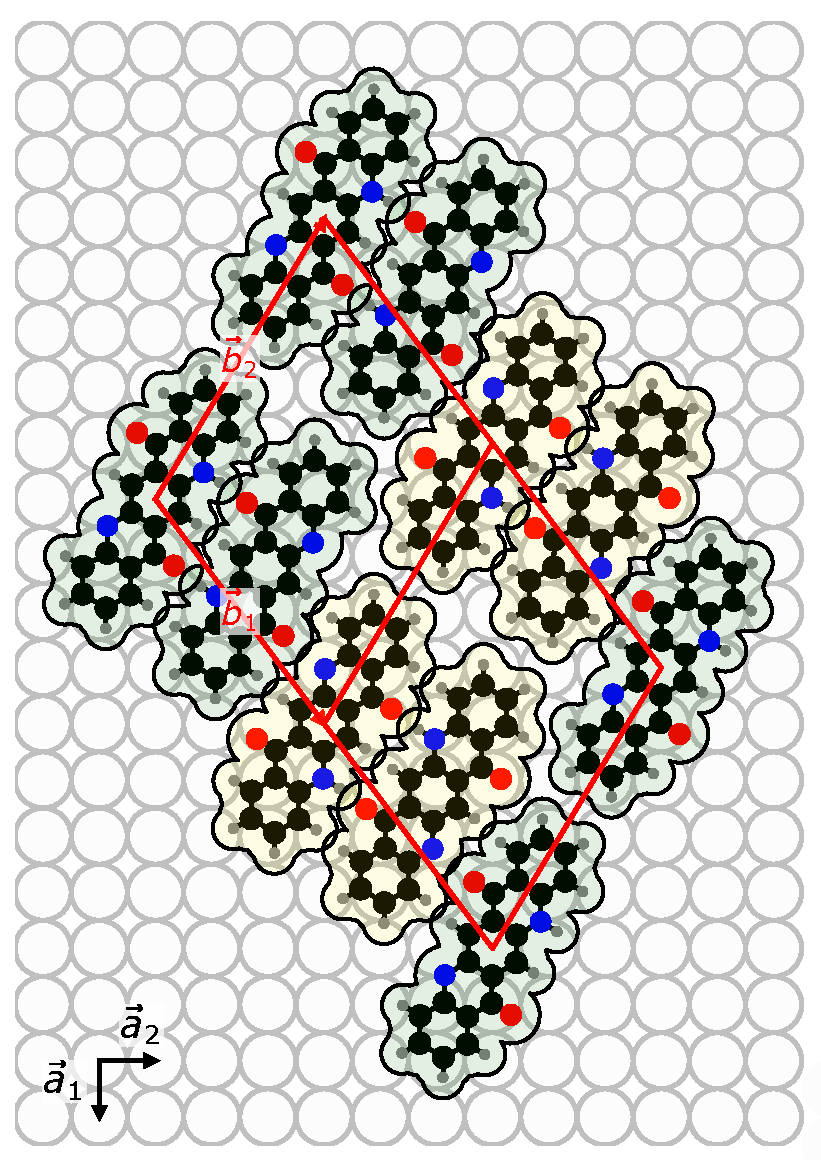
\includegraphics[width=\linewidth]{images/QA-beta-Ag(100)-Version1.pdf}}
	\end{subcaptionbox}
	\hfill
	\begin{subcaptionbox}{structure model 2}[0.49\linewidth]
		{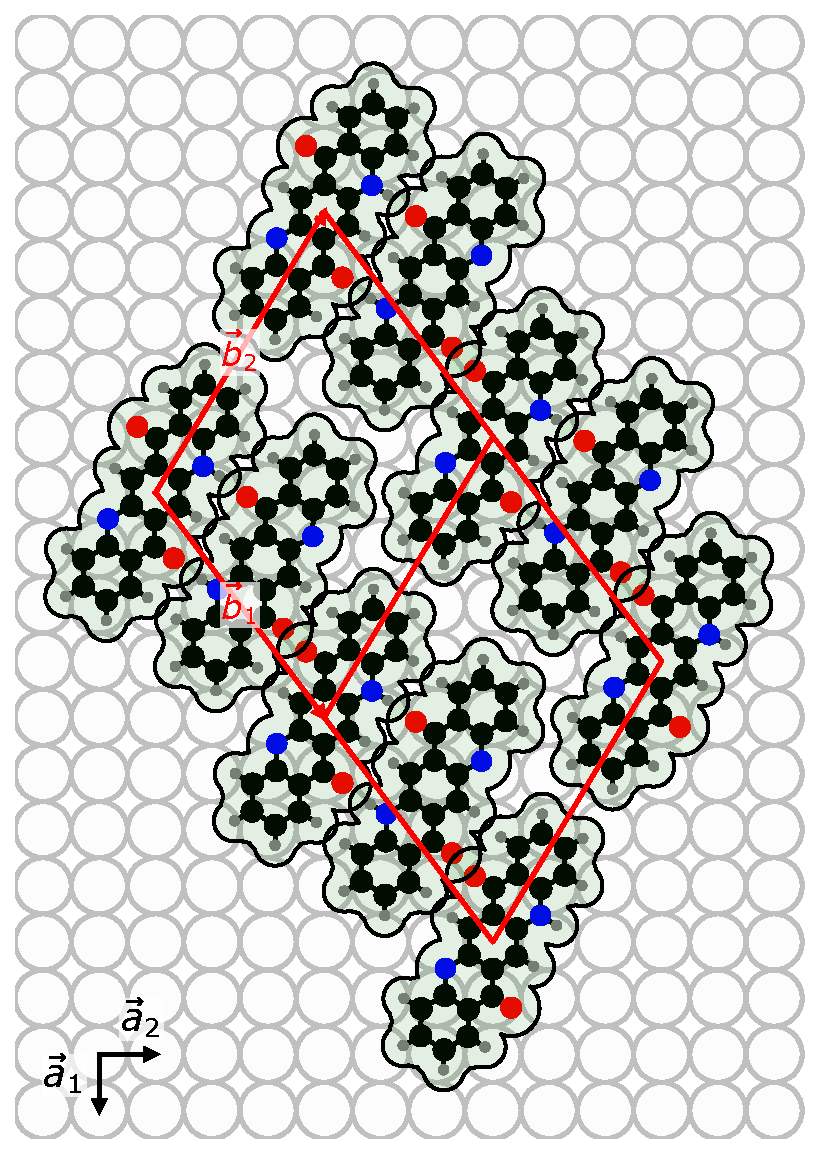
\includegraphics[width=\linewidth]{images/QA-beta-Ag(100)-Version2.pdf}}
	\end{subcaptionbox}
	\caption{Two different structure models for the $\beta$-phase of \ac{QA} on Ag(100).}
	\label{fig:models}
\end{figure}

The second structure model has more changes compared to the one of N. Humberg.\autocite{Humberg2024} Instead of the heterochiral dimers, the structure model is homochiral. This means that the molecules do not have to rotate on the surface for the phase transition from the $\alpha$- to the $\beta$-phase. The model also forms the same amount of hydrogen bridges as model 1.

However, a significant issue has been identified with model 2. As depicted in the structure model, the oxygen atom of one molecule is directly opposite to the oxygen atom of another molecule. The plausibility of this occurrence appears to be minimal, because they should also repel each other. It could also be possible that both oxygen atoms approach the surface and donate electron density to the surface. This could increase the distance between the atoms and decrease the repulsion. Nevertheless, model 2 appears to be less probable than model 1 for the reasons previously enumerated.

\cleardoublepage


\chapter{Summary and Outlook}

In summary, the present study has expanded the understanding of the phase behaviour of \ac{QA} on Ag(100) by examining the $\alpha$- and the $\beta$-phase in greater detail. The investigation of the $\alpha$- and the $\beta$-phase was conducted by utilizing \ac{XPS} for the C1s, N1s and O1s components.

The results for the $\alpha$-phase are consistent with the prior findings by N. Humberg.\autocite{Humberg2024} The proposed structure model has been be confirmed. In addition, all \ac{XPS} spectra, particularly those of the C1s core-level, can be subdivided into multiple peaks and allocated to particular atoms of \ac{QA}. Furthermore, the consequences of beam damage due to exposure of \ac{QA} to the x-ray were investigated. The results demonstrated that the deprotonation of the amine group occured as a result of this exposure.

A subsequent examination of the results for the $\beta$-phase reveals inconsistencies with the proposed structure model by N. Humberg\autocite{Humberg2024} for this phase. It was ascertained that the $\beta$-phase is composed of two distinct oxygen atoms, exhibiting a stoichiometric ratio of 1~:~1. A comparable observation was made in the case of the nitrogen atoms. Additionally, it was determined that deprotonation of one of the nitrogen atoms is necessary due to its shift in binding energy, leading to only one hydrogen bond per molecule. The findings of this study have led to the proposition of the novel structure model in \autoref{fig:models}.

Nevertheless, the extant structure models leave unresolved questions in need of further investigation. To further refine our comprehension of \ac{QA} on Ag(100), it is imperative to undertake additional research to develop a more detailed structure model. Therefore, \ac{NIXSW} measurements could be used to determine the adsorption height of the atoms, which allow a revision of the structure model. Beyond that, different \ac{NIXSW} measurements could be used for triangulation of the $\beta$-phase. This should give exact adsorption sites for the atoms and allow a detailed structure model.

\cleardoublepage
\chapter{Appendix}
\label{sec:appendix}
\raggedbottom

\begin{figure}[H]
	\centering
	\includegraphics[height=0.95\textwidth, angle=90]{images/C1s-all.png}
	\caption{Collection of all C1s core-level \ac{XPS} spectra with the different fitted peaks of all performed experiments. Each spectrum corresponds to a different preperation. The coverage of the first spectrum is set to 1~\ac{ML}.}
	\label{fig:C1s-stacked}
\end{figure}

\begin{figure}[H]
	\centering
	\includegraphics[width=0.85\textwidth]{images/O1s-all.png}
	\caption{Collection of all O1s core-level \ac{XPS} spectra with the different fitted peaks of all performed experiments. Each spectrum corresponds to a different preperation. The coverage of the first spectrum is set to 1~\ac{ML}.}
	\label{fig:O1s-stacked}
\end{figure}

\begin{figure}[H]
	\centering
	\includegraphics[height=0.9\textwidth,  angle=90]{images/N1s-all.png}
	\caption{Collection of all N1s core-level \ac{XPS} spectra with the different fitted peaks of all performed experiments. Each spectrum corresponds to a different preperation. The coverage of the first spectrum is set to 1~\ac{ML}.}
	\label{fig:N1s-stacked}
\end{figure}


\newpage
\section*{List of abbreviations}
\addcontentsline{toc}{section}{List of abbreviations}

\begin{acronym}
    \acro{Ag}[Ag]{silver}
    \acro{BE}[BE]{binding energy}
    \acro{fcc}[fcc]{face-centered cubic}
    \acro{FWHM}[FWHM]{full width at half maximum}
    \acro{LEED}[LEED]{low energy electron diffraction}
    \acro{ML}[ML]{monolayer}
    \acro{NIXSW}[NIXSW]{normal incidence x-ray standing wavefield absorption}
    \acro{OFET}[OFET]{organic field-effect transistor}
    \acro{OLED}[OLED]{organic light-emitting diode}
    \acro{OPV}[OPV]{organic photovoltaic}
    \acro{POL}[POL]{point-on-line}
    \acro{PTCDA}[PTCDA]{perylenetetracarboxylic dianhydride}
    \acro{QA}[QA]{quinachridone}
    \acro{SPA-LEED}[SPA-LEED]{spot profile analysis low energy electron diffraction}
    \acro{STM}[STM]{scanning tunneling microscopy}
    \acro{UHV}[UHV]{ultra-high vacuum}
    \acro{XPS}[XPS]{x-ray photoelectron spectroscopy}
\end{acronym}

\acrodefplural{BE}{binding energies}




\printbibliography[heading=bibintoc]
\end{document}